\documentclass[../../main.tex]{subfiles}

\begin{document}
\fexercisesHeader

\exercise{4.1}
\begin{wts}
    If $\card{\xx}\geq 2$, there is a topology on $\xx$ that is $T_0$ but not $T_1$.
\end{wts}
\begin{proof}
    Let $\Tau_\xx = \{\varnothing\}\cup\{\{x\}\cup B,\: B\subseteq \xx\}$, where $x\in\xx$ is any point in $\xx$. Suppose $U_1$, and $U_2$ are open sets in $\Tau_\xx$, if either is empty then their intersection must be contained in $\Tau_\xx$. Otherwise $U_1 = \{x\}\cup B_1$, and $U_2 = \{x\}\cup B_2$, where $B_1$ and $B_2$ are subsets of $\xx$.
    \[
        U_1\cap U_2 = \{x\}(B_1\cap B_2)\in \Tau_\xx
    \]
    Notice also $\{\varnothing,\: \xx\}\subseteq\Tau_\xx$. Fix an arbitrary family of open sets $\{U_\alpha\}_{\alpha\in A}$, in similar fashion we have $\bigcup U_\alpha = \{x\}\cup\biggl( \bigcup B_{\alpha\in A} \biggr)$ so their union is contained in $\Tau_\xx$ as well.\\

    This topology is $T_0$. Fix $y\neq z$ in $\xx$, if either $y$ or $z$ is $x$, then choosing $\{x\}$ does the job. So assume $x\neq y\neq z\neq x$, and $\{y\}\cup \{x\}$ is an open set that does not contain $z$. This topology cannot be $T_1$, as $x$ sticks onto every open set, so there are no open sets which separate $x$ from the other points in $\xx$.
\end{proof}
\newpage

\exercise{4.2}
\begin{wts}
    If $\xx$ is an infinite set, the cofinite topology on $\xx$ is $T_1$ but not $T_2$, and is first countable iff $\xx$ is countable.
\end{wts}
\begin{proof}
    We will first verify that the cofinite topology $\Tau_\xx$ is a topology. 
    \[
        \Tau_\xx = \bigset{U,\quad U^c \text{ is finite.}}\cup \{\varnothing\}
    \]
    So that $\{\varnothing,\: \xx\}\subseteq\Tau_\xx$. Let $U_1$ and $U_2$ be a pair of open sets, assuming if neither of them are empty, then $U_2^c$ and $U_1^c$ are finite sets, so that $U_1^c\cup U_2^c$ is finite as well. Use DeMorgan to see that $U_1\cap U_2\in\Tau_\xx$.\\

    If $\{U_\alpha\}_{\alpha\in A}$ is an arbitrary collection of open sets, then 
    \[
        \bigcap_{\alpha\in A} U_\alpha^c\subseteq U_\beta^c
    \]
    where $\beta\in A$ is arbitrary, so $U_\beta^c$ is finite. And the union $\bigcup U_\alpha$ is contained in $\Tau_\xx$.\\

    To show that $\Tau_\xx$ is $T_1$, every singleton set is closed. To show that $\Tau_\xx$ is not $T_2$, fix $x\neq y$. If $B_x$ and $B_y$ are open sets that contain $x$ and $y$ respectively. If $B_x$ and $B_y$ disjoint, then 
    \[
        B_x\subseteq B_y^c
    \]
    Which means $B_x$ is an open, finite subset. But the only open and finite subset of $\xx$ is the empty set. This contradicts $x\in B_x$.\\

    If $\xx$ is countable, we will find a neighbourhood base $\nb{x}$ for any $x \in \xx$ as follows: 
    \begin{itemize}
        \item We can index $\xx$ using $\nat^+\cup\{0\}$, so without loss of generality, let $x_0 = x$, and 
        \item Define $U_1 = \{x_1\}^c$, and $U_n = \bigcap_{j=1}^n \{x_j\}^c$ are open sets that contain $x$. Equivalently,
        \[
            U_n = \bigset{x_j,\: j\geq n+1}\cup\{x_0\}
        \]
        \item If $V$ is an open set that contains $x_0$, then $V^c$ is finite, let $M\in\nat^+$ be the largest index of $x_j\notin V$ (the negation of this is that if $j\geq M+1$, then $x_j\in V$) then $U_{M+1}\subseteq V$ as needed, and $\xx$ is first countable.
    \end{itemize}
    Conversely, if $\xx$ is first countable, we can find a descending sequence of neighbourhoods which form a neighbourhood base, $\{U_j\}_{j\geq 1}\subseteq \Tau_\xx$. And each $U_j^c$ is finite, so $\bigcup U_j^c$ is countable. Assume for contradiction that $\xx$ is uncountable, then 
    \[
        \bigcup U_j^c = \biggl(\bigcap U_j\biggr)^c
    \]
    is countable, hence the intersection $\bigcap U_j$ must be uncountable (hence infinite). Pick $y\neq x$, where $y$ belongs in the intersection of all neighbourhoods $U_j$. This contradicts the fact that $\{U_j\}$ is a neighbourhood base, as $x$ is an element in the open set $\{y\}^c$ therefore there must be a $U_k$ 
    \[
        x\in U_k\subseteq \{y\}^c
    \]
    But $y\in U_k$ for each $U_k$ and the proof is complete.
\end{proof}

\newpage

\exercise{4.3}
\begin{wts}
    Every metric space is normal. (If $A,B$ are disjoint closed sets in the metric space, consider the set of points $x$ where $d(x,A)< d(x,B)$ or $d(x,A)> d(x,B)$).
\end{wts}
\begin{proof}
    First, we show that if $A$ is closed, then $d(x,A) = 0\iff x\in A$. If $x\in A$, then $d(x,A)\leq d(x,x) = 0$. if $x\notin A$, then there exists a ball of radius $\varepsilon>0$ where $B(\varepsilon, x)\cap A = \varnothing$. Hence, $\varepsilon$ is a lower bound for the set $\{d(x,y),\: y\in A\}$, taking the infimum over this set we see that $d(x,A)\geq \varepsilon>0$.\\

    Fix some $x\in \Phi_A$ where $\Phi_A = \bigset{y\in\xx, d(y,A) < d(y,B)}$. We wish to find an open ball about $x$ that is contained in $\Phi_A$. The Triangle Inequality works for this definition of distance as well, as
    \begin{equation}\label{eq:function-infimum}
        f(a)\leq g(a), \forall a\in A\implies \inf_{a\in A}f(a)\leq \inf_{a\in A}g(a)
    \end{equation}
    If $a\in A$, then $d(z,A)\leq d(x,z) + d(x,A)$, using \Cref{eq:function-infimum} yields 
    \[
        \begin{cases}
            d(z,A)\leq d(x,A) + d(x,z)\\
            d(x,B)-d(x,z)\leq d(z,B)
        \end{cases}
    \]
    where $z\in B(\varepsilon, x)$ so $d(x,z)\lsim\varepsilon$. The second estimate above is found by 'flipping an upper bound to become a lower bound'. We can choose $d(x,z)$ sufficiently small that 
    \[
        d(x,A) + d(x,z) < d(x,B) - d(x,z)
    \]
    in order to 'pipe' the two inequalities, so
    \begin{equation}\label{ex:4.3-distance-estimate}
        2d(x,z) < d(x,B) - d(x,A)
    \end{equation}
    Take $\varepsilon = [d(x,B) - d(x,A)]3^{-1}$, then $z\in B(\varepsilon, x)$ implies $d(x,z)<\varepsilon$, and \Cref{ex:4.3-distance-estimate} holds. See \Cref{fig:ex4.3} for details.\\
\begin{figure}
    \centering
    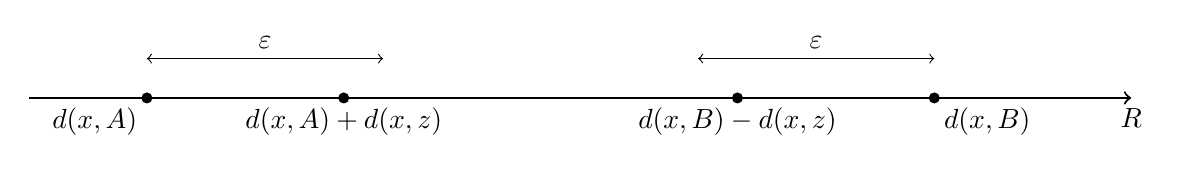
\begin{tikzpicture}
    % Draw the real line
    \draw[thick,->] (-0.5,0) -- (13.5,0) node[below] {$\mathbb{R}$};
    
    % Left Markers
    \fill (1,0) circle (2pt);
    \fill (3.5,0) circle (2pt);
    \node[below left] at (1,0) {$d(x,A)$};
    \node[below] at (3.5,0) {$d(x,A) + d(x,z)$};
    \draw[<->] (1,0.5) -- (4,0.5) node[midway,above] {$\varepsilon$};

    % Right Markers
    \fill (8.5,0) circle (2pt);
    \fill (11,0) circle (2pt);
    \node[below right] at (11,0) {$d(x,B)$};
    \node[below] at (8.5,0) {$d(x,B) - d(x,z)$};
    \draw[<->] (8,0.5) -- (11,0.5) node[midway,above] {$\varepsilon$};
\end{tikzpicture}
    \caption{Exercise 4.3: Finding a $\varepsilon$ small enough that fits within $d(x,A) < d(x,B)$}
    \label{fig:ex4.3}
\end{figure}
\end{proof}
\newpage

\exercise{4.4}
\begin{wts}
    
\end{wts}
\begin{proof}
    
\end{proof}
\newpage


\exercise{4.5}
\begin{wts}
    Every separable metric space is second countable.
\end{wts}
\begin{proof}
    We wish to show that if $\xx$ is a metric space, then
    \[
        \text{second countable } \iff \text{ separable}
    \]
    Suppose $\xx$ is separable, where $A$ is a countable dense subset in $\xx$, and $x\in\xx$. Let $U$ be an open set that contains $x$, so $B(\varepsilon,\: x)\subseteq U$ for some $\varepsilon>0$. $B(\varepsilon/2,\: x)$ is a non-empty open set, therefore contains some $y\in A$ (this follows from the definition of density). If we choose $r\in \mathbb{Q}$ wisely,
    \[
        d(x,y) < r < \varepsilon/2
    \]
    So that $x\in B(r,\: y)$, and if $z\in B(r,\: y)$, then 
    \[
        d(x,z)\leq d(x,y) + d(z,y)< r + r < \varepsilon
    \]
    So $x \in B(r,\: y)\subseteq U$. But $\{B(r,y),\: r\in\rat^+,\: y\in A\}$ is countable. Therefore $\xx$ is second countable.\\
    
    Conversely, Proposition 4.5 gives us the $\impliedby$ direction. But we will repeat anyway, if $\xx$ is second-countable with $\Epsilon$ as a countable base, then take 
    \[
        W = \bigset{x_\alpha\in U,\quad U\in \Epsilon}
    \]
    by picking a point from each set, we claim $W$ is dense in $\xx$, so $\cl{W}=\xx$. If not, then $\cl{W}^c \neq\varnothing$, and 
    \[
        \cl{W}^c = (W^c)^o \neq \varnothing
    \]
    Pick a point $x \in W^{co}$, which is an open set containing $x$. But the way we chose $W$ does not allow for any open set $U\in \Epsilon$ with $x\in\Epsilon \subseteq W^{co}$, since
    \begin{quote}
        By picking one point from each of the base sets, and flipping the complement. We can ensure that no $U\in\Epsilon$ from the countable base is fully contained as a subset of $W^{co}$, as there is always one point from each $U\in\Epsilon$ that cannot be found in $W^{co}$
    \end{quote}
\end{proof}
\newpage

\exercise{4.6}
\begin{wts}
\end{wts}
\begin{proof}
    
\end{proof}
\newpage

\exercise{4.7}
\begin{wts}
    If $\xx$ is a topological space, a point $x\in\xx$ is called a cluster point of the sequence $\{x_j\}$ if for every neighbourhood $U\in\N{x}$, $x_j\in U$ for infinitely many $j$. If $\xx$ is first countable, $x$ is a cluster point of $\{x_j\}$ iff some subsequence of $\{x_j\}$ converges to $x$.
\end{wts}
\begin{proof}
    Suppose $\{x_n\}$ has a cluster point in $z\in \xx$. Fix a descending sequence of neighbourhoods $U_k\subseteq \N{z}$, where
    \[
        U_1\supseteq U_2\supseteq\cdots\supseteq U_k
    \]
    Define $n_k = \least\bigset{j\in \natplus,\: j>n_{k-1},\: x_j\in U_k}
    $ with $n_0=0$, so that for every $m\geq k$, $x_{n_m}\in U_k$ eventually. And $\{x_{n_j}\}_{j\geq 1}$ is a subsequence which converges to $z$. This proves ($\implies$).\\
    
    Conversely (this part does not require that $\xx$ be first countable, if $\{x_{n_k}\}_{k\geq 1}$ is a subsequence that converges to $z\in\xx$. Every neighbourhood of $z$ must intersect all but infinitely many $x_{n_k}$, therefore $z$ is a cluster point of $\{x_n\}$.
\end{proof}
\newpage




\exercise{4.8}
\begin{wts}
    If $\xx$ is an infinite set with the cofinite topology and $\{x_j\} $ is a sequence of distinct points in $\xx$, then $x_j\to x$ for every $x\in\xx$.   
\end{wts}
\begin{proof}
    The intuition here is that the cofinite topology does not distinguish between points, so it acts as a type of jelly that hides the points.\\

    Let $x\in\xx$ be arbitrary, if $U\in\N{x}$ then $U^o\in\N{x}$, so that $\{y_j\}_{j\leq k}$ are the $k$ points that are required to extend $U^o$ to $\xx$. (All but finitely many points are in any open set of $\xx$).\\

    There exists a large $N\in\natplus$ so that for every $n\geq N$, 
    \[
        x_j\notin\{y_j\}_{j\leq k}\implies x_j\in U^o
    \]
    eventually. And $x_j\to x$.
\end{proof}
\newpage

\exercise{4.9}
\begin{wts}
    
\end{wts}
\begin{proof}
    
\end{proof}
\newpage

\exercise{4.10}
\begin{wts}
    A topological space $\xx$ is called disconnected if there exists non-empty, disjoint open sets $U$, $V$ and $U\cup V = \xx$; otherwise $\xx$ is connected. When we speak of connected or disconnected subsets of $\xx$, we refer to the relative topology on them
    \begin{enumalpha}
        \item $\xx$ is connected iff $\varnothing$ and $\xx$ are the only two clopen sets.
        \item If $\{E_\alpha\}_{\alpha\in A}$ is a collection of connected subsets of $\xx$, and $bigcap E_{\alpha\in A}$ is non-empty, then $\bigcup E_{\alpha\in A}$ is connected.
        \item If $A\subseteq\xx$ is connected, then $\cl{A}$ is connected,
        \item Every point in $x\in\xx$ contained in a unique maximal connected subset of $\xx$, and this subset is closed. It is called the connected component of $x$.
    \end{enumalpha}
\end{wts}
\begin{proof}
    The proof is rather long, so we will split it in several parts. A topological space is disconnected iff it can be written as a disjoint union of two non-empty open sets. Often it is easier to show that a space is disconnected rather than connected.\\

    Part A: Suppose $\xx$ is disconnected, this induces a pair of non-empty open sets, $A$, and $B$ whose union is $\xx$, and 
    \[
        A\cap B = \varnothing\iff A \subseteq B^c
    \]
    their union is $\xx$, hence
    \[
        A\cup B = \xx\iff B^c\subseteq A
    \]
    combining the last two estimates, we see that $B = A^c$, so both $A$ and $A^c = B$ are closed. This proves ($\impliedby$).\\
    Now suppose $\{A, A^c\}\neq \{\varnothing,\xx\}$ are both clopen. Clearly $A$ is disjoint from its complement, and their union is $\xx$.\\

    Part B: We will attempt the contrapositive. Suppose $E = \bigcup E_{\alpha\in A}$ is disconnected. This induces $D$ and $D^c$ which are clopen in the relative topology of $E$, (by Part A). More precisely,
    \begin{equation}\label{chp4:ex4.10-union-non-empty}
        \bigcup E_\alpha = \underbrace{\bigcup (E_\alpha\cap D)}_{\neq\varnothing} + \underbrace{\bigcup (E_\alpha\setminus D)}_{\neq\varnothing}
    \end{equation}
    The intersection $\bigcap E_{\alpha\in A}$ is non-trivial, hence
    \begin{equation}\label{chp4:ex4.10-intersection-non-empty}
        \bigcap E_\alpha = \underbrace{\bigcap (E_\alpha\cap D)}_{\neq\varnothing} + \bigcap (E_\alpha\setminus D) \neq\varnothing
    \end{equation}    
    so at least one of the members on the right are non-empty. Assume without loss of generality that $\bigcap (E_\alpha\cap D)$ is not empty. This tells us $E_\alpha\cap D=\neq\varnothing$ for each $\alpha\in A$. But by \Cref{chp4:ex4.10-union-non-empty}, if we concentrate on the right member, 
    \[
        \bigcup (E_\alpha\setminus D)\neq\varnothing\implies\exists\beta\in A,\: E_\alpha\setminus D \neq\varnothing
    \]
    And for this particular $\beta\in A$, we see that both $D$ and $D^c$ are non-trivially open in $E_\beta$, and the proof is complete. A poetic way to summarize the proof would be:
    \begin{quote}
        If the whole is disconnected, and there exists common ground over which the family of sets covers, and because the common ground (intersection) is non-trivial, either $D$ or $D^c$ is non-trivially open in all $E_\alpha$. The intersection gives us "$\forall$", while the union gives us "$\exists$" for a non-trivially open $D$ or $D^c$.
    \end{quote}

    Part C: Suppose $\cl{A}$ is disconnected, this induces a non-trivial clopen set $D$ relative to $\cl{A}$. 
    \begin{itemize}
        \item Since $\cl{A}\cap D\neq\varnothing$, choose any $y\in\cl{A}\cap D\subseteq \cl{A}$, since $D$ is a neighbourhood of $y$, and $y$ is an adherent point of $A$. It is immediate that $A\cap D$ is non-empty.
        \item Similarly for $A\setminus D\neq\varnothing$,
    \end{itemize}
    therefore $\{D,D^c\}$ is non-trivially clopen in $A$, and $A$ is disconnected.\\

    Part D: The idea here is to use Part B. Let $x$ be fixed, and $\{E_\alpha\}_{\alpha\in A}$ be the family of all connected sets containing $x$, since their intersection is non-trivial, their union, $E$ is connected. The closure of their union is then the maximal connected component containing $x$. Indeed, if $G$ is a connected set containing $x$, then $G\subseteq \bigcup E_\alpha = E$, so $G\subseteq \cl{E}$.
\end{proof}
\newpage

\exercise{4.11}
\begin{wts}
    If $E_1,\ldots E_n$ are subsets of a topological space, the closure of $\bigcup_1^n E_j$ is $\bigcup_1^n \cl{E_j}$
\end{wts}
\begin{proof}
    The finite union of closed sets is again closed, so 
    \[
        \forall j\leq n,\: E_j\subseteq \cl{E_j}\implies \cl{\bigcup_1^n E_j}\subseteq \bigcup_1^n \cl{E_j}
    \]
    For the reverse estimate, $E_j\subseteq\bigcup_1^n E_j\subseteq \cl{\bigcup_1^n E_j}$ is a closed set that contains each $E_j$, therefore
    \[
        \forall j\leq n,\: \cl{E_j}\subseteq \cl{\bigcup_1^n E_j}\implies \bigcup_1^n \cl{E_j}\subseteq \cl{\bigcup_1^n E_j}
    \]
\end{proof}
\begin{corollary}
    The interior operator distributes over intersections. If $A$ and $B$ are subsets of $\xx$, then
    \begin{align*}
        \cl{(A^c\cup  B^c)} &= (\cl{A^c}\cup \cl{B^c})\\
        \biggl(\cl{(A^c\cup  B^c)}\biggr)^c&= A^o\cap B^o\\
        \biggl(A^c\cup B^c\biggr)^{co} &= A^o\cap B^o\\
        (A\cap B)^o&=A^o\cap B^o
    \end{align*}
\end{corollary}
\newpage

% Kuratowski Closure Operaotrs
\exercise{4.12}
\begin{wts}
    Let $\xx$ be a set. A Kuratowski closure operator on $\xx$ is a map $A\mapsto A^*$ from $\powerset{\xx}$ to itself satisfying
    \begin{enumroman}
        \item $\varnothing^* = \varnothing$ (does nothing to the empty set),
        \item $A\subseteq A^*$ (monotonicity),
        \item $(A^*)^* = A^*$ (idempotence)
        \item $(A\cup B)^* = A^* \cup B^*$ (distributes over finite unions)
    \end{enumroman}
    Prove
    \begin{enumalpha}
        \item If $\xx$ is a topological space, the map $A\mapsto \cl{A}$ is a Kuratowski closure operator. (Use Exercise 11.)
        \item Conversely, given a Kuratowski closure operator, let $\mathcal{F} = \{ A\subseteq \xx,\: A = A^*\}$ and $\Tau = \{U\subseteq \xx,\: U^c\in \mathcal{F}\}$, then $\Tau$ is a topology on $\xx$, and for any set $A\subseteq\xx$, $A^*$ will be its closure with respect to $\Tau$.
    \end{enumalpha}
\end{wts}
\begin{proof}
    Part A: The empty set is closed, so $\cl{\varnothing}=\varnothing$, and $\cl{A}$ is the smallest closed superset of $A$, so $A\subseteq\cl{A}$ for every $A\subseteq\xx$. $A\subseteq\xx$ is closed iff $\cl{A} = A$, so idempotence holds. Distributivity follows from Exercise 11 directly.\\

    Part B: We first show that $\Tau$ is indeed a topology. Fix $U_1$ and $U_2$ in $\Tau$, so that $U_1^c\cup U_2^c = (U_1\cap U_2)^c$. The map $A\mapsto A^*$ distributes over finite unions, hence 
    \[
        (U_1^c \cup U_2^c)^* = (U_1^c)^* \cup (U_2^c)^* = U_1^c\cup U_2^c
    \]
    Therefore $U_1\cap U_2\in \Tau$. Now suppose $\{U_\alpha\}_{\alpha\in A}\subseteq\Tau$, then
    \[
        \biggl( \bigcup U_\alpha\biggr)^c = \bigcap U_\alpha^c
    \]
    by monotonicity (Property ii): $\bigcap U_\alpha^c\subseteq\biggl(\bigcap U_\alpha^c\biggr)^*$. To prove the reverse inclusion, notice if $\alpha$ is held fixed,
    \[
        \bigcap U_\alpha^c\subseteq U_\alpha^c\implies \biggl(\bigcap U_\alpha^c\biggr)^*\subseteq U_\alpha^{c*}
    \]
    this follows from 'monotonicity' of the closure operator: if $A$ is a subset of $B$, then we can write 
    \[
        B = A + (B\setminus A)\implies A^* \subseteq A^* + (B\setminus A)^* = B^*
    \]
    Take the intersection over all $\alpha\in A$ on the right member,
    \[
        \biggl(\bigcap U_\alpha^c\biggr)^*\subseteq \bigcap U_\alpha^{c*} = \bigcap U_\alpha^c
    \]
    Hence $\biggl(\bigcap U_\alpha^c \biggr)^* = \bigcap U_\alpha^c $. The empty set and $\xx$ are elements of $\mathcal{F}$. Since $\xx\subseteq \xx^*\subseteq \xx$, and $\{\varnothing,\xx\}\subseteq\Tau$. So $\Tau$ is a topology.\\

    Finally, $A^*$ is a closed superset of $A$ and suppose $K$ is another closed superset,
    \[
        A \subseteq K\implies A^*\subseteq K^*
    \]
    So $A^*$ is the smallest closed superset of $A$ and this proves the last claim.
\end{proof}
\newpage




\exercise{4.13}
\begin{wts}
    If $\xx$ is a topological space, $U$ is open in $\xx$ and $A$ is dense in $\xx$, then $\cl{U} = \cl{U\cap A}$.
\end{wts}
\begin{proof}
    The takeaway here is that if $A$ is dense in $\xx$, every point $z\in U$ can be approximated by points in $U\cap A$. And and important technique of 'demoting' the neighbourhood to become the interior of the neighbourhood can yield some nice properties. Since the interior of a neighbourhood is again a neighbourhood. This allows intersection with open sets to inherit the 'neighbourhoodness' of the set.\\

    Let $z\in \cl{U}$, and fix a neighbourhood $V\in \N{z}$, so that the interior of $V$ is also a neighbourhood. By the alternate definition of $\cl{U}$ in terms of adherent points (see \Cref{chp4:closure-adherent}) of $\cl{U}$, $V^o\cap U\neq\varnothing$. This is a non-empty open set, therefore it must intersect $A$ non-trivially.
    \[
        x\in (V^o\cap U)\cap A = V^o\cap (U\cap A)
    \]
    and $z\in \cl{U\cap A}$.\\
\end{proof}
\begin{remark}
We simply used the fact 
\[
\cl{E} = \bigset{x\in\xx,\: \forall V\in\N{x},\: V\cap E\neq\varnothing}
\]
and the following equivalent characterization of density
\[
E \text{ is dense in }\xx \iff \text{ For every non-empty open set } U,\: U\cap E\neq\varnothing
\]
\end{remark}
\newpage


\exercise{4.14}
\begin{wts}
    If $\xx$ and $\yy$ are topological spaces, $f: \xx\to\yy$ is continuous iff $f(\cl{A})\subseteq\cl{f(A)}$ for every $A\subseteq \xx$ iff $\cl{f^{-1}(B)}\subseteq f^{-1}(\cl{B})$ for all $B\subseteq Y$.
\end{wts}
\begin{proof}
    \emph{First Equivalence:} If $f$ is continuous, fix any $A\subseteq\xx$, and $z\in \cl{A}$, by \Cref{chp4:closure-adherent} (I will spare you the flipping by including):
    \[
    \cl{A} = \{x\in\xx,\: \forall U\in\N{X},\: U\cap A\neq\varnothing\}
    \]
    Let $U\in \N{f(z)}$, so that $f^{-1}(U^o)$ is an open set containing $z$ and $f^{-1}(U^o)\in\N{z}$, so
    \[
        f^{-1}(U^o)\cap A\neq\varnothing\implies U^o\cap f(A)\subseteq U\cap f(A)
    \]
    so $f(\cl{A})\subseteq \cl{f(A)}$. Conversely, suppose $f(\cl{A})\subseteq\cl{f(A)}$ holds for every $A\subseteq\xx$. The following is a sequence of symbolic manipulations that I found but have zero intuitive understanding about. First take the inverse image
    \[
        \cl{A}\subseteq f^{-1}\biggl(f(\cl{A})\biggr)\subseteq f^{-1}\biggl(\cl{f(A)}\biggr)
    \]
    Next, let $F$ be a closed set in $\yy$, and make the substitution $A = f^{-1}(F)$, hence
    \[
        \cl{f^{-1}(F)}\subseteq f^{-1}\biggl(\cl{f(f^{-1}(F))}\biggr)\subseteq f^{-1}(\cl{F})=f^{-1}(F)
    \]
    for the second inclusion we used the monotonicity of the closure, and since $\cl{f^{-1}(F)} = f^{-1}(F)$, we are done.
    \\

    \emph{Second Equivalence:} Suppose $f\in C(\xx,\yy)$, then $\cl{B}\subseteq \yy$ is a closed set, so $f^{-1}(\cl{B})$ is closed in $\xx$. By monotonicity of the inverse image,
    \[
        f^{-1}(B)\subseteq f^{-1}(\cl{B})\implies \cl{f^{-1}(B)}\subseteq f^{-1}(\cl{B})
    \]
    Conversely, if $\cl{f^{-1}(B)}\subseteq f^{-1}(B)$ for any $B\subseteq \yy$, take any closed $B\subseteq \yy$, and 
    \[
        \cl{f^{-1}(B)}\subseteq f^{-1}(B)\subseteq \cl{f^{-1}(B)}
    \]
    so $f^{-1}(B)$ is closed, and $f$ is in $C(\xx,\yy)$.
\end{proof}
\newpage


\exercise{4.16}
\begin{wts}
\end{wts}

\begin{proof}
    \begin{enumalpha}
        \item[]
        \item Let $x\in \{f\neq g\}$, then there exists disjoint open subsets of $\yy$, $f(x)\in U$ and $g(x)\in V$, $U\cap V=\varnothing$, but $f^{-1}(U)\cap g^{-1}(V)$ is an open set in $\xx$ that contains $x$. Therefore $\{f\neq g\}$ is open in $\xx$.
        \item Suppose $\{f=g\}=E$ is dense in $\xx$. Let $x\in E$, induces two disjoint open sets exactly like in part a. This is an open set that contains $x$, and $y\in f^{-1}(U)\cap g^{-1}(V)\cap E$. Since $y\in E$, it follows that $f(y) = g(y)$, and
        \[
            \begin{cases}
            y\in f^{-1}(U)\implies &f(y)\in U\\
            y\in g^{-1}(V)\implies &g(y)\in V
            \end{cases}
        \]
    \end{enumalpha}
\end{proof}
\newpage


\exercise{4.17}



\end{document}